\chapter{Password Strength}

The password strength is determined by calculating entropy of the 
password. An entropy is described in terms of bits. The higher the bits in entropy
the stronger the password will be. An entropy indicates how hard it will be to 
crack the password by brute-force. In password strength calculation, the entropy 
is not the same entropy as described in information theory. Rather the raw entropy 
is lowered by using various password cracking techniques before accepting.

\section{Understanding Password Entropy}
Entropy in password security measures the unpredictability and strength of a password. There are two main approaches to calculating password entropy:
\begin{enumerate}
    \item \textbf{Raw Entropy}: This method calculates entropy based solely on the password's length and character set. It often results in higher entropy values, which some password strength tools use.
    
    \item \textbf{Adjusted Entropy}: Our tool uses this more nuanced approach. We start with the raw entropy, then apply various reduction techniques to account for real-world password vulnerabilities.
\end{enumerate}

\section{Why Our Entropy Scores Might Seem Lower}

Our tool provides a more conservative and realistic assessment of password strength. We apply several techniques to reduce the initial entropy, including:

\begin{itemize}
    \item NIST Special Publication 800-63 guidelines
    \item Weakening for repeated characters
    \item Adjustments for lowercase-only passwords
    \item Qwerty keyboard pattern recognition
    \item Dictionary word detection
    \item Leet speak translation (e.g., ``@'' to ``a'')
    \item Keyboard pattern adjustments
\end{itemize}
For example, in our tests:
\begin{itemize}
    \item ``Tr0ub4dor\&3'' has a raw entropy of 72.27, but an adjusted entropy of 19.63
    \item ``correcthorsebatterystaple'' starts at 117.51 and adjusts to 30.95
    \item ``password'' goes from 37.60 to 2.0
\end{itemize}

These adjustments reflect real-world vulnerabilities that attackers might exploit, providing a more accurate representation of your password's strength against modern cracking techniques.

While our entropy scores may appear lower than other tools, they offer a more realistic assessment of your password's security in practical scenarios. Always aim for higher entropy scores and follow good password creation practices for optimal security.

\section{Entropy Calculation}
This section describes the basics of entropy calculation. Please note that we
do not calculate password or passphrase entropy this way, rather we
use various password cracking techniques to lower the raw entropy and if the
entropy is higher or equal to the configured entropy, only then the password
is accepted.

If the password length is $L$ and the password can be chosen from $N$ number of
characters, the possible number of passwords will be $N^L$. To calculate the raw 
entropy $H$ in that character space, the $H$ has to be a number so that
$2^H = N^L$. Therefore, the entropy calculation formula can be derived as follows:

\begin{align}
                 2^H &= N^L\label{eq:1} \\
           \log(2^H) &= \log(N^L)\label{eq2}\\
    H \times \log(2) &= L \times \log(N)\label{eq:3}\\
                   H &= L \times \frac{\log(N)} {\log(2)}\label{eq:4} \\
                     &= L \times \log_{2}(N)\label{eq:5}
\end{align}
\footnotetext[1]{$\log{_b}(x^p) = p\log{_b}(x)$}
\footnotetext[2]{$\log_{b}(x) = \frac{\log(x)}{\log(b)}$}

Given a password entropy $H$ and the number to guess a password per second is ($gps$), the time in seconds
$T_{s}$ to brute force a password can be calculated with the following formula:

\begin{align*}
    T_{s} &= \frac{2^H} {gps}
\end{align*}

The following xkcd comic illustrates entropy calculation of password in a 
different way.

\begin{figure}[H]
    \centering
    \fbox{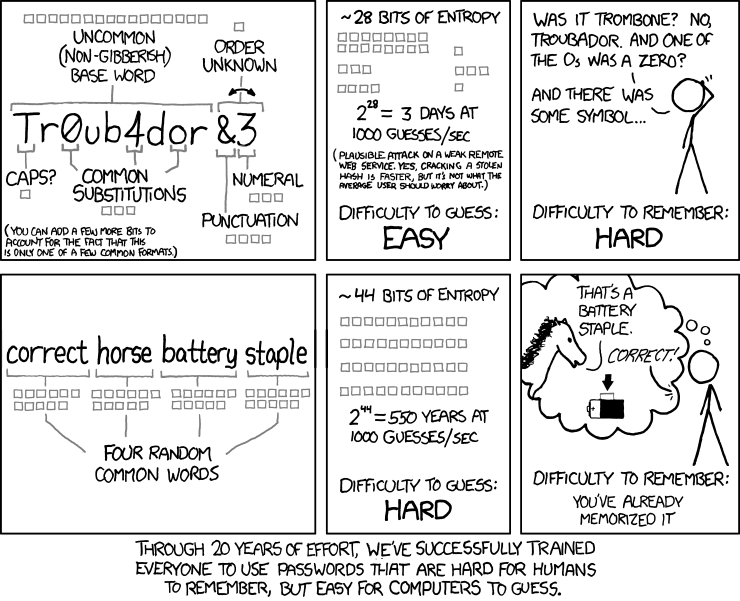
\includegraphics[scale=0.6]{common/xkcd_password_strength.png}}
    \caption{xkcd comic for password strength}
    \label{fig: Figure}
\end{figure}

Let's calculate the entropy of \texttt{Tr0ub4dor\&3} with our formula
$H = L \times \log_{2}(N)$. The password has upper case, lower case, numbers and a 
special character in it. There are 26 upper case, 26 lower case, 10 numbers and
32 special characters (including space) in English keyboard and the length $L$ of the password is 
$11$. 

\begin{align*}
    N &= 26 + 26 + 10 + 32 = 94 \\
    H &= 11 \times \frac{\log(94)} {\log(2)} =  72.10047736845401109442 \approx 72
\end{align*}
Assuming that the attacker knows the length of the password $L$ and character
space $N$,
if $gps = 1000$, it will take $\frac{2^{72}} {1000}$ $\approx$ $150\ billion$ years 
to crack the password. If $gps =350\ billion$, it will take $\approx$ $428$ years to crack 
the password. if $gps = 1\ trillion$, it will take $\approx 150\ years$ to crack the
password. So if brute force is used, it is really a good password, even with the
most powerful computer, it will take a long time to crack. 

According to xkcd,
the password is not strong, lets see how xkcd calculates the entropy. Each of
the tiny square box in the comic indicates a bit. 
\begin{itemize}
    \item The $16$ bits implies that the word 
\texttt{Troubador} is chosen from a dictionary with $65536$ words ($2^{16} = 65536$).
    \item Make the first letter upper case, there is only $1\ bit$.
    \item Two characters were substituted $o \rightarrow 0$, $a \rightarrow 4$ and $o$ was
not substituted, therefore $3 bits$ of information.
    \item The string \texttt{\&3} was appended at the end. The order is unknown, therefore $1\ bit$
    \item There are 32 special characters (including space) in English keyboard, therefore the entropy should
be $1 \times \frac{\log(32)} {\log(2)} = 5$. For some reason $4 bit$ was selected.
\end{itemize}


Therefore, the entropy of \texttt{Tr0ub4dor\&3} is $ 16 + 1 + 3 + 1 + 4 + 3 = 28$, which much 
is lower than 72 and makes it a bad password, because the attacker might follow
the similar technique than brute-forcing it.

\section{Entropy calculation in Obidos}
The technique we used in Obidos, the entropy for the password \texttt{Tr0ub4dor\&3}
comes down to 19.625. we used similar techniques used the ruby gem 
\href{https://github.com/bdmac/strong_password}{strong\_password}

\begin{enumerate}
    \item Calculate entropy according to
\href{https://nvlpubs.nist.gov/nistpubs/Legacy/SP/nistspecialpublication800-63ver1.0.2.pdf}{NIST Special Publication 800-63 Version 1.0.2} Appending A.2.1
    \begin{itemize}
        \item The first character gets 4 bits
        \item The next 7 characters get 2 bits/character
        \item The next 12 characters (9-20) get 1.5 bits/character
        \item Any character beyond 20 gets 1 bit/character
        \item If there are mixed case and special character, give 6 bits bonus
    \end{itemize}
    Using these rules, the entropy of \texttt{Tr0ub4dor\&3} comes down to 26.125
    \item Calculate the entropy by lowering the case, which is also 26.125
    \item Adjust entropy by checking if the password has any pattern of 
Qwerty keyboard (e.g. zxcvbn, qwertyuiop etc.) which is 26.125
    \item Adjust the entropy by looking at dictionary, doing normal
substitutions like xkcd, checking for leet speak pattern etc. The entropy comes down
to 19.625.
    \item Finally select the lowest entropy, which is 19.625 
\end{enumerate}
The entropy of \texttt{correcthorsebatterystaple} comes down to 30.953125 which
is much lower than xkcd's 44 bit entropy.
\section{Suggestions for strong passwords}
Please think passphrase when picking a password. Passphrases are longer and 
easier to remember than a cryptic random password which is difficult to remember.
The longer the password is, the stronger it will be. Refer to the equation \eqref{eq:5}.
\begin{itemize}
    \item Think passphrase. The longer, the better! Avoid using repeating characters
    \item Use a line from a poem or a song and mix with Upper, lower case letters and numbers
    \item Use uncommon words. Capitalization does not help much
    \item Add typos, space, special characters \! \@ \# \$ \% \textasciitilde \ \textasciicircum \ \& \* \( \) etc. here and there.
If the password is a long passphrase, there is no requirement to use any 
special character. However, your organization might have a password policy 
that requires them.
    \item Do not use username, email, phone numbers etc.
\end{itemize}
\section{Password storage}
A password is never stored in the disk, rather a memory-hardened, brute-
force resisting key is derived from the given password and a stored salt. To verify a 
password, the same key is derived from the password and the salt and 
compared.  The function deriving the key from the password and
the salt is CPU intensive and intentionally requires a fair amount of 
memory. Therefore, it mitigates brute-force attacks by requiring a 
significant effort to verify each password. 

The password is hashed using
\href{https://github.com/P-H-C/phc-winner-argon2/raw/master/argon2-specs.pdf}{Argon2id} algorithm. 
